\subsection{Build a simple DCGAN}

As well as creating a simple VAE, we implement a simple convolutional \textit{Generative Adversarial Network} (GAN) following the DCGAN model that we are first going to train on the MNIST dataset.

The following structure is implemented. The discriminator is composed of two 2D convolutional layers and two linear layers. On the first three layers, we compute a batch normalization and a Leaky ReLU activation. The generator is build symmetrically with three transpose 2D convolutional layers followed by batch normalization and a ReLU activation, and finally a last convolutional layer with a Tanh activation. 

Firstly we use a Binary Cross Entropy (BCE) loss, as used in the original paper, and an Adam optimizer on both the discriminator and the generator. 

In order to avoid instabilities due to vanishing gradient or mode collapse issues, in a second time we replace the BCE loss by a Least Square GAN (LSGAN) loss. 

\begin{figure}
    \centering
    \begin{subfigure}[b]{\textwidth}
        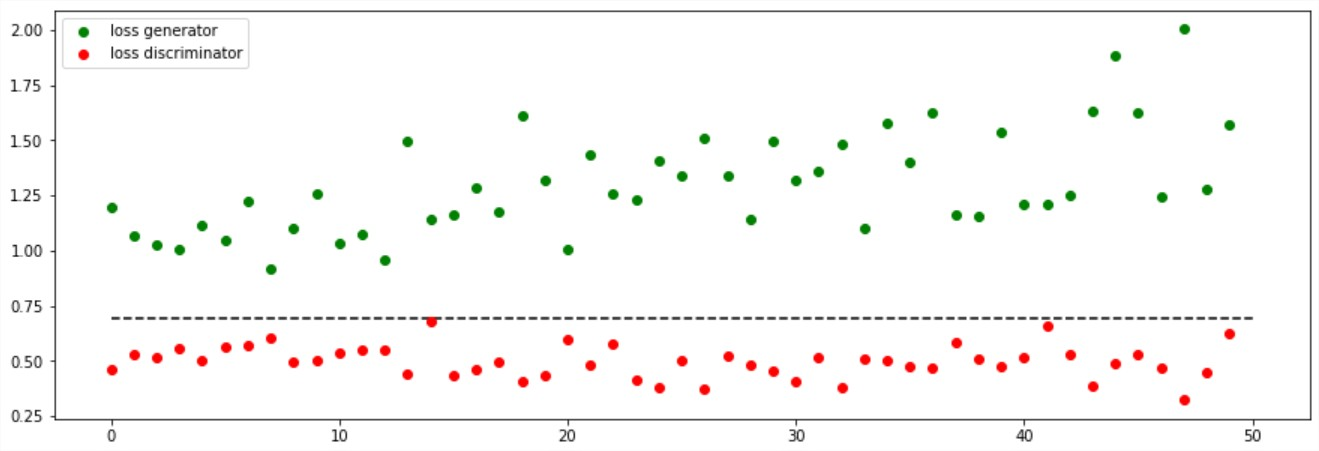
\includegraphics[width=\linewidth]{simple_dcgan/loss_BCE.jpg}
        \caption{BCE loss}
    \end{subfigure}
    \begin{subfigure}[b]{\textwidth}
        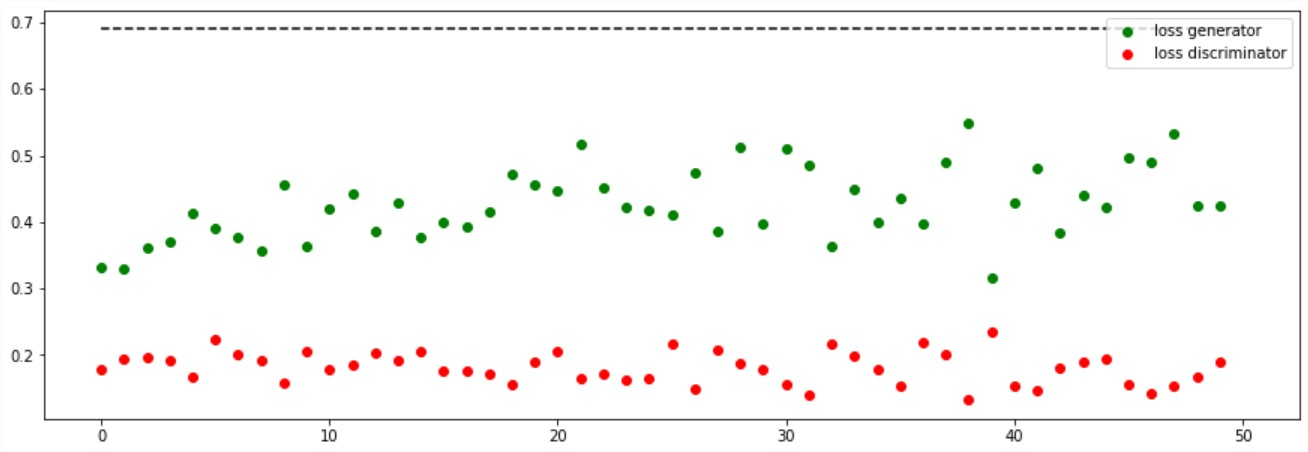
\includegraphics[width=\linewidth]{simple_dcgan/loss_MSE.jpg}
        \caption{MSE loss (Least Square)}
    \end{subfigure}
    \caption{}
    \label{fig:my_label}
\end{figure}